\documentclass[11pt]{article}

\usepackage[margin=1in]{geometry}
\usepackage{amsmath, amssymb}
\usepackage{graphicx}
\usepackage{booktabs}
\usepackage{hyperref}
\usepackage{listings}
\usepackage{xcolor}

\title{MPES Computation Workflow \\ 21-Node Grid}
\author{Team Technical Documentation}
\date{}

\begin{document}
\maketitle

\section{Overview}

This document describes the workflow used to compute the Maximum Power Energy Section (MPES) for a 21-node grid using a weighted Max-Cut formulation.

\section{Mathematical Formulation}

Let the grid be an undirected weighted graph:

\[
G = (V, E, w)
\]

The cut weight is:

\[
\text{Cut}(S) = \sum_{(i,j)\in E} w_{ij} \cdot \mathbf{1}[i \in S, j \notin S]
\]

The MPES is:

\[
\text{MPES} = \frac{\text{Cut}(S^*)}{\sum_{(i,j)\in E} w_{ij}}
\]

\section{Computation Pipeline}

\subsection{Exact Optimal Cut}

For 21 nodes, half-enumeration guarantees the global optimum.

\subsection{Plateau Verification}

We verify local optimality using k-flip checks:

\[
S' = S \oplus F, \quad |F| \leq 4
\]

If $\text{Cut}(S') \leq \text{Cut}(S)$ for all $F$, the solution is locally stable.

\subsection{Trust Metrics}

We compute:

\begin{itemize}
\item Load balance
\item Redundancy
\item N-1 resilience
\item Bottleneck ratio
\end{itemize}

\section{Results}

\begin{tabular}{ll}
\toprule
Metric & Value \\
\midrule
Nodes & 21 \\
Edges & 28 \\
Cut Value & 3728.4132 \\
MPES & 0.8844 \\
Trust Score & 0.9382 \\
Plateau (k $\leq$ 4) & TRUE \\
\bottomrule
\end{tabular}

\section{Figures}

\subsection{Partition Visualization}

\begin{figure}[h]
\centering
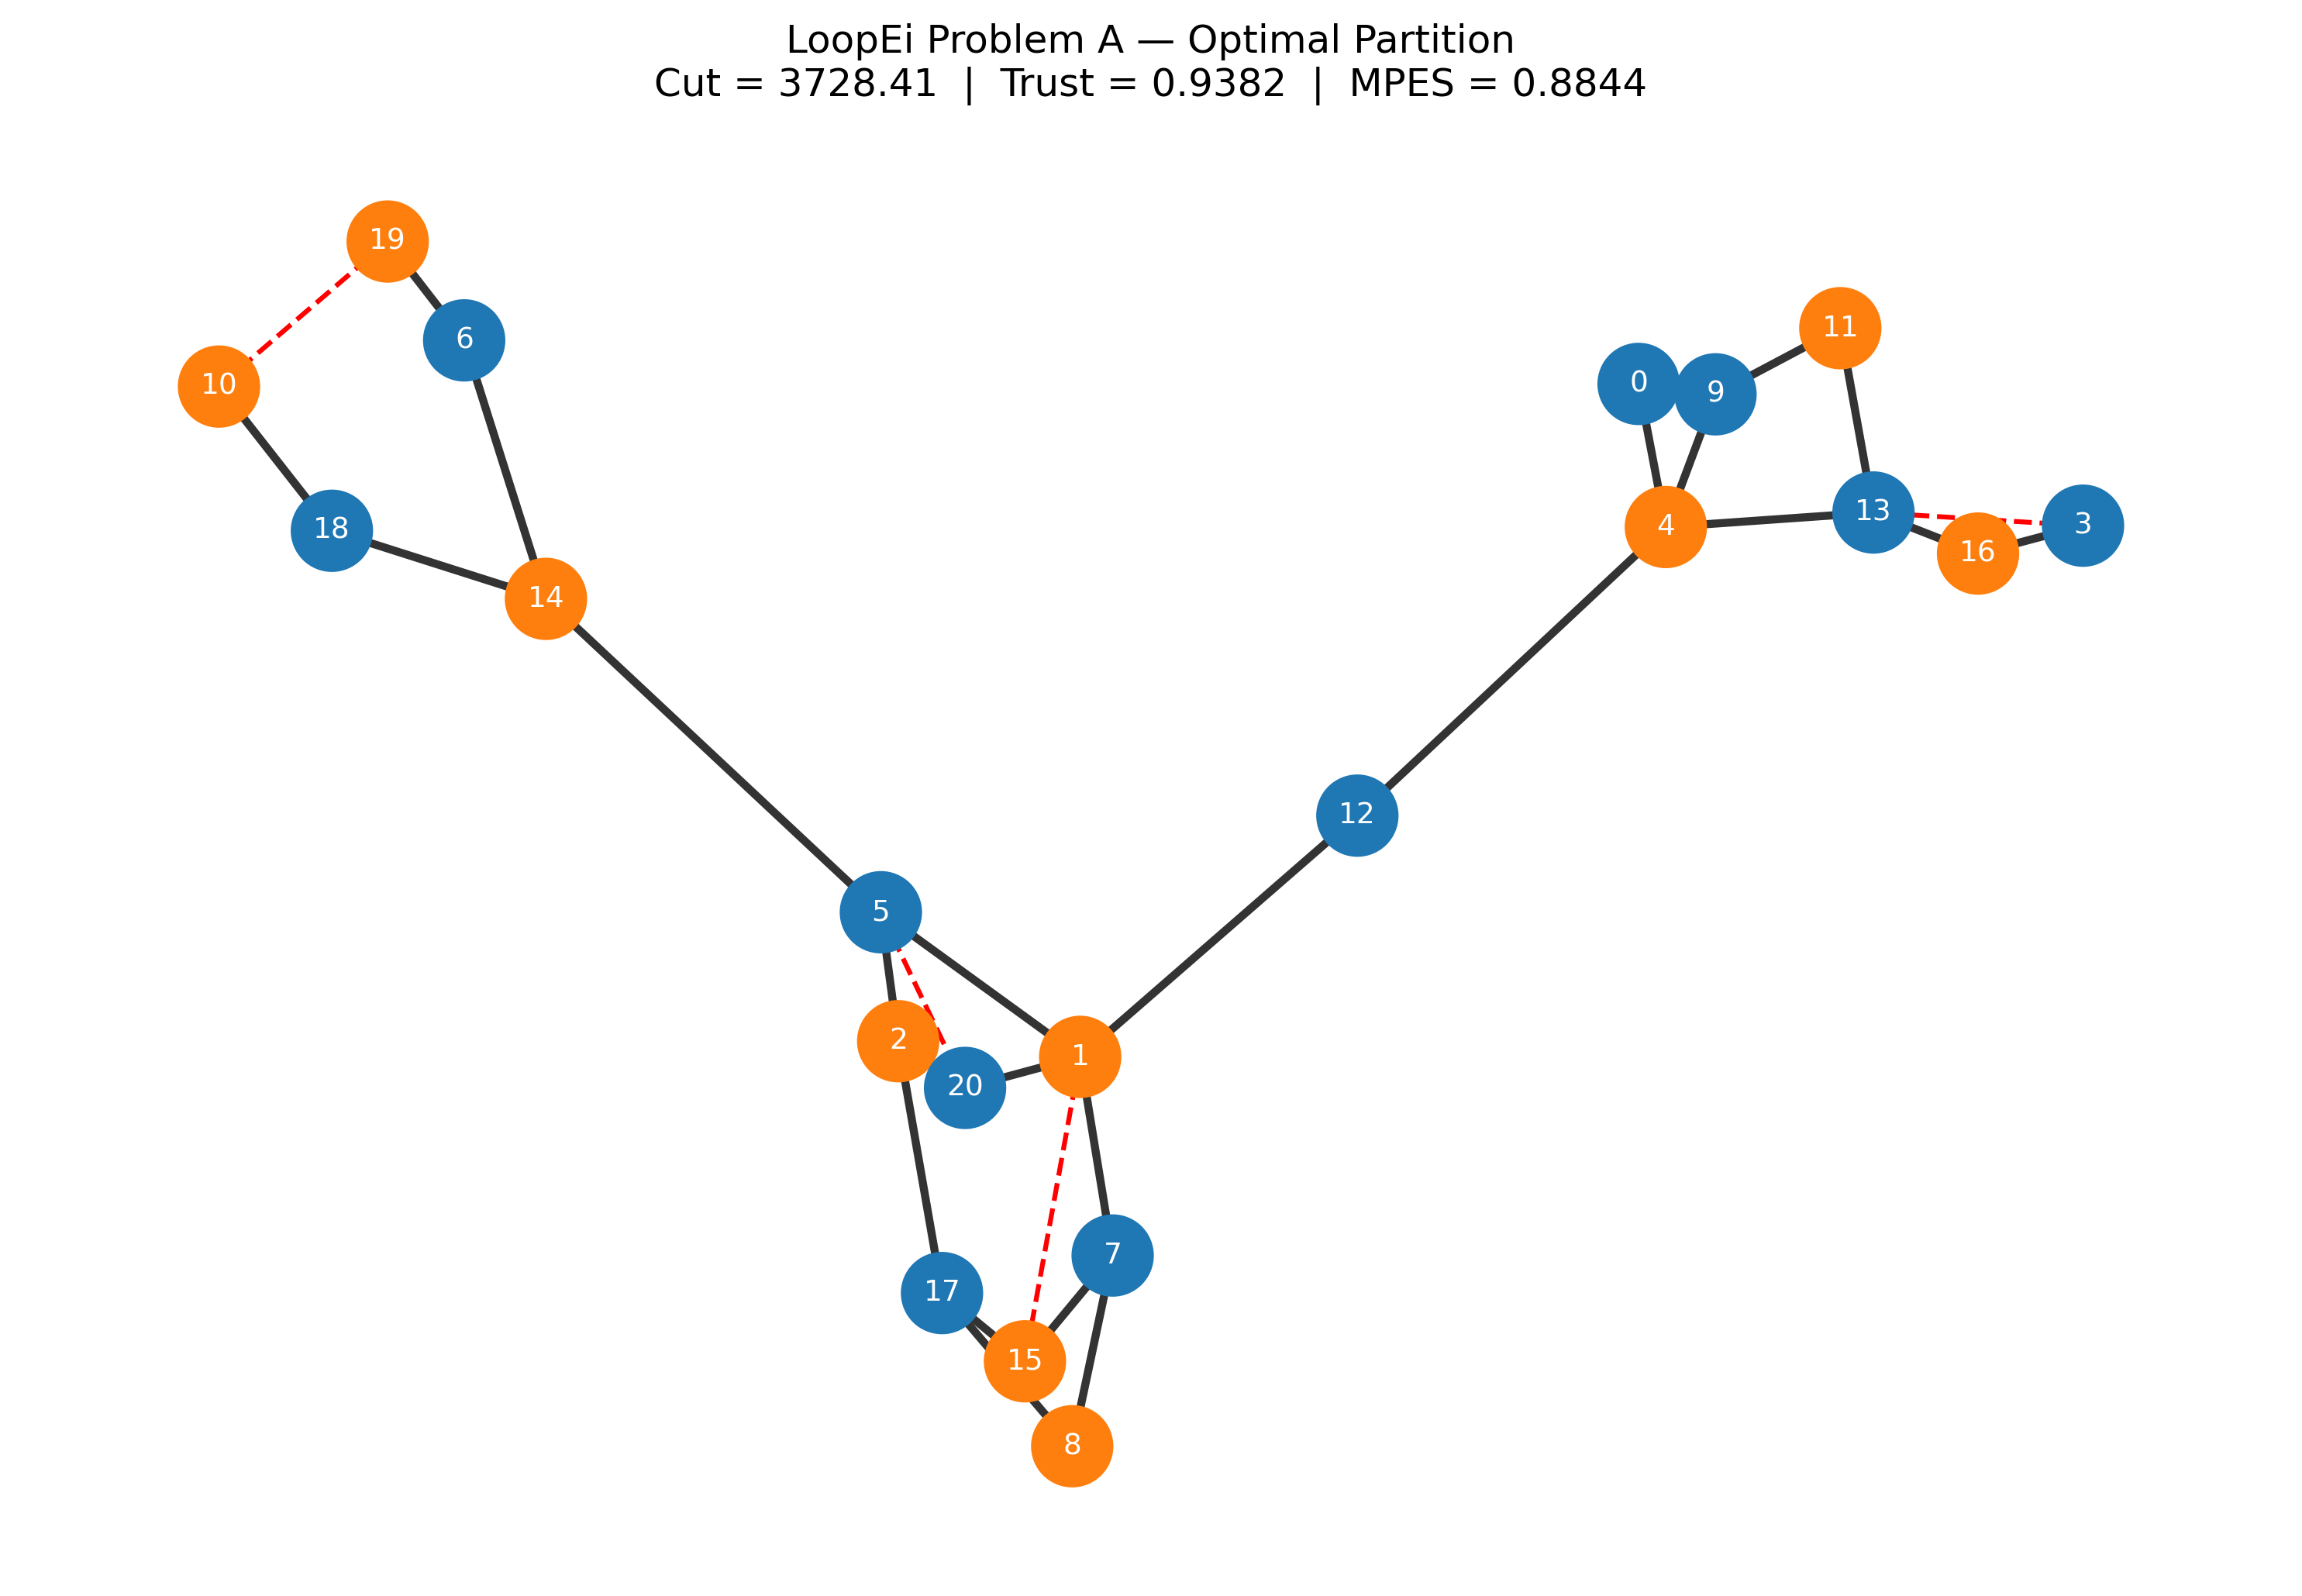
\includegraphics[width=0.7\textwidth]{partition_plot.png}
\caption{Optimal partition of the grid}
\end{figure}

\subsection{MPES Histogram}

\begin{figure}[h]
\centering
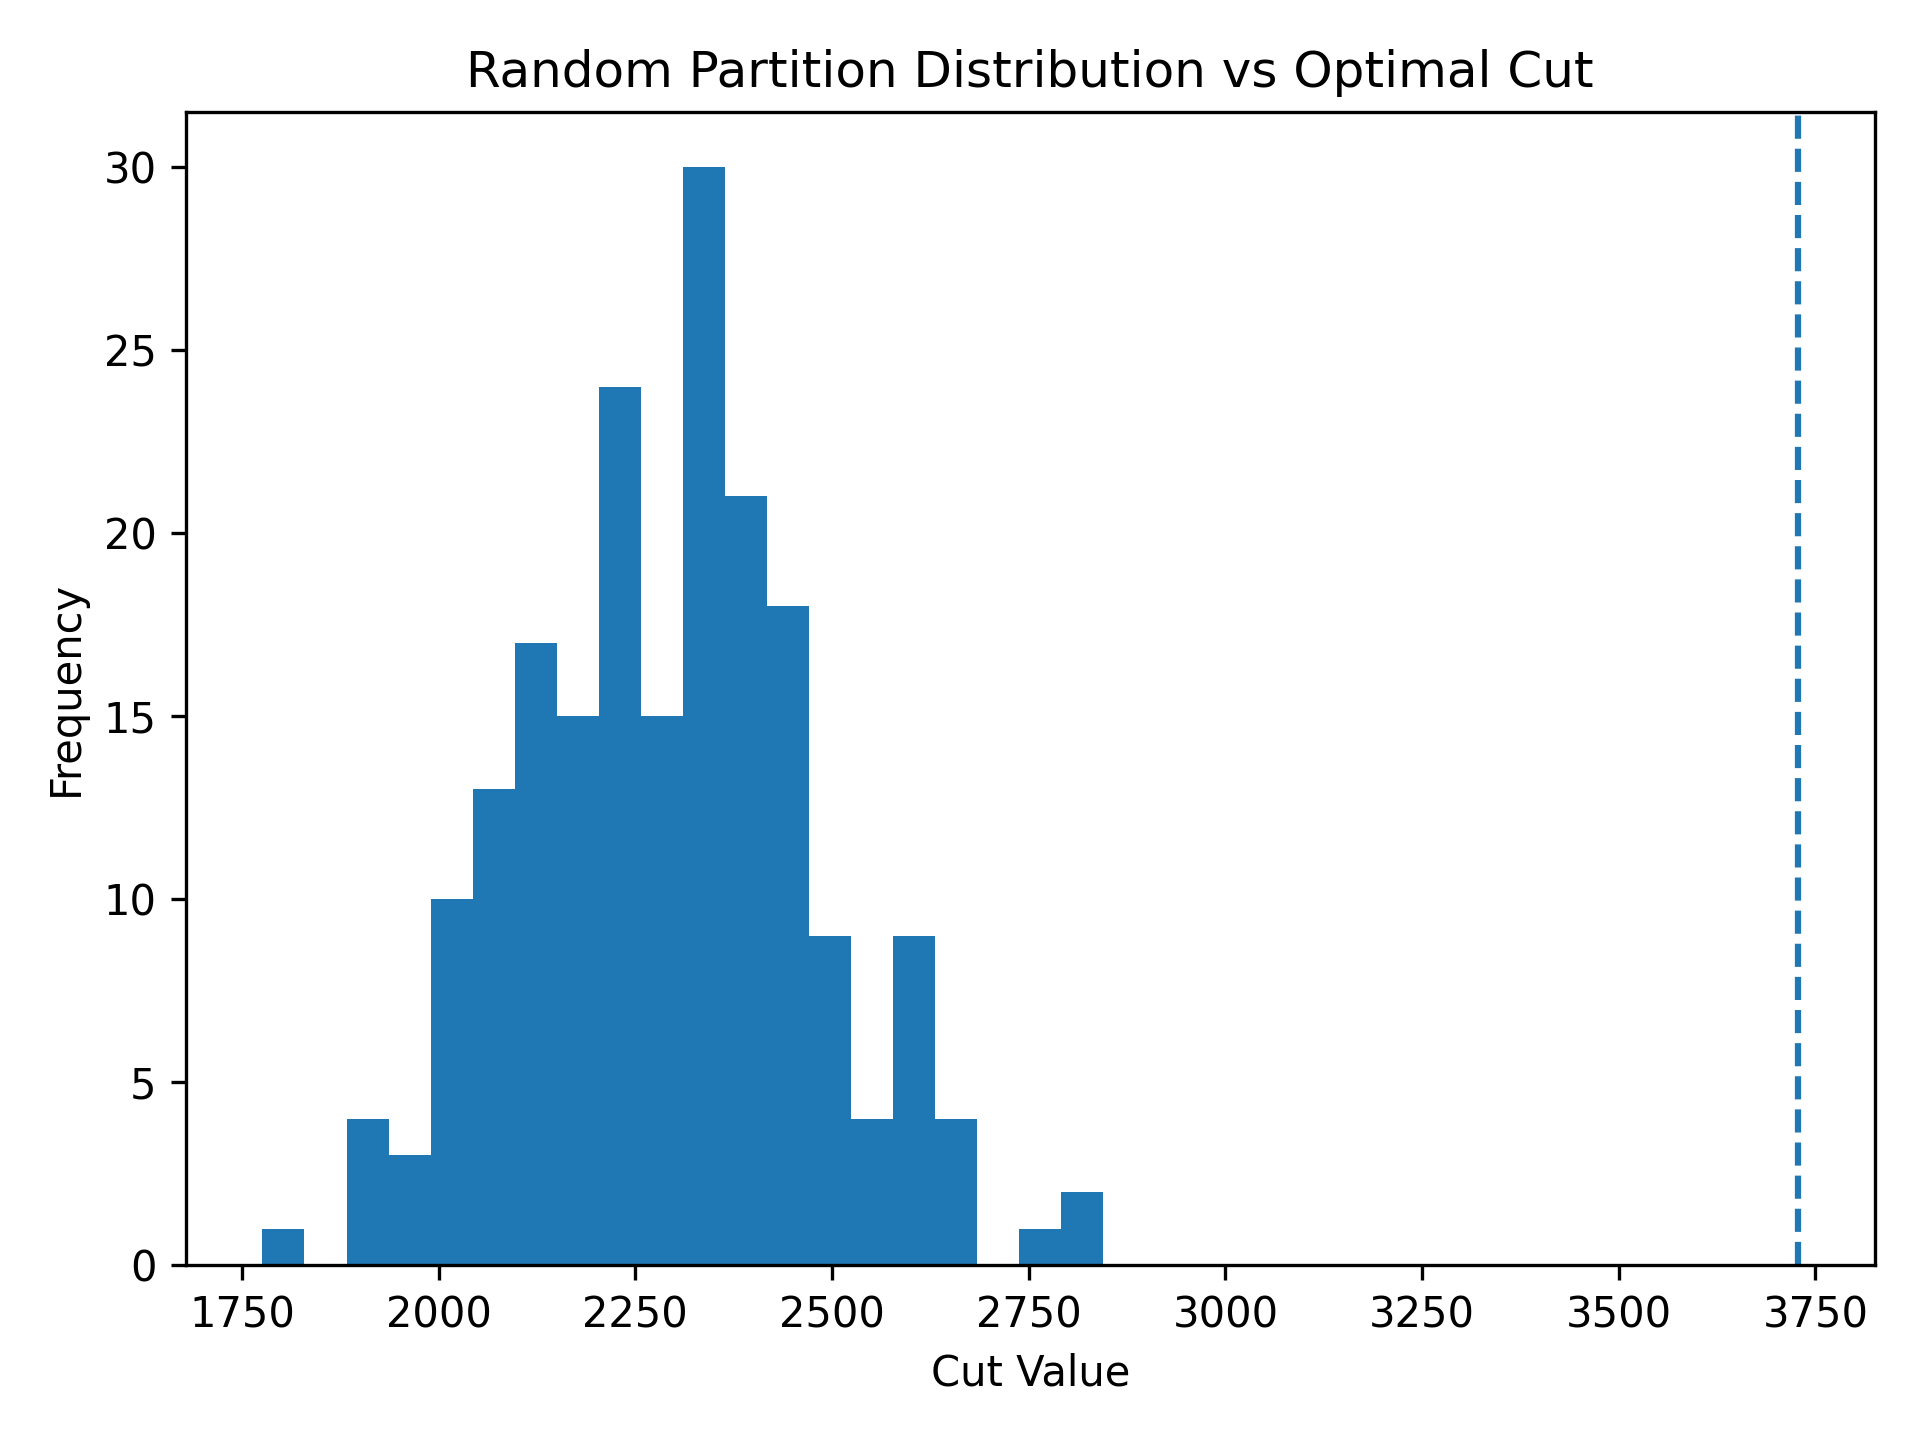
\includegraphics[width=0.7\textwidth]{mpes_histogram.png}
\caption{Distribution of MPES across sampled partitions}
\end{figure}

\subsection{Plateau Verification}

\begin{figure}[h]
\centering
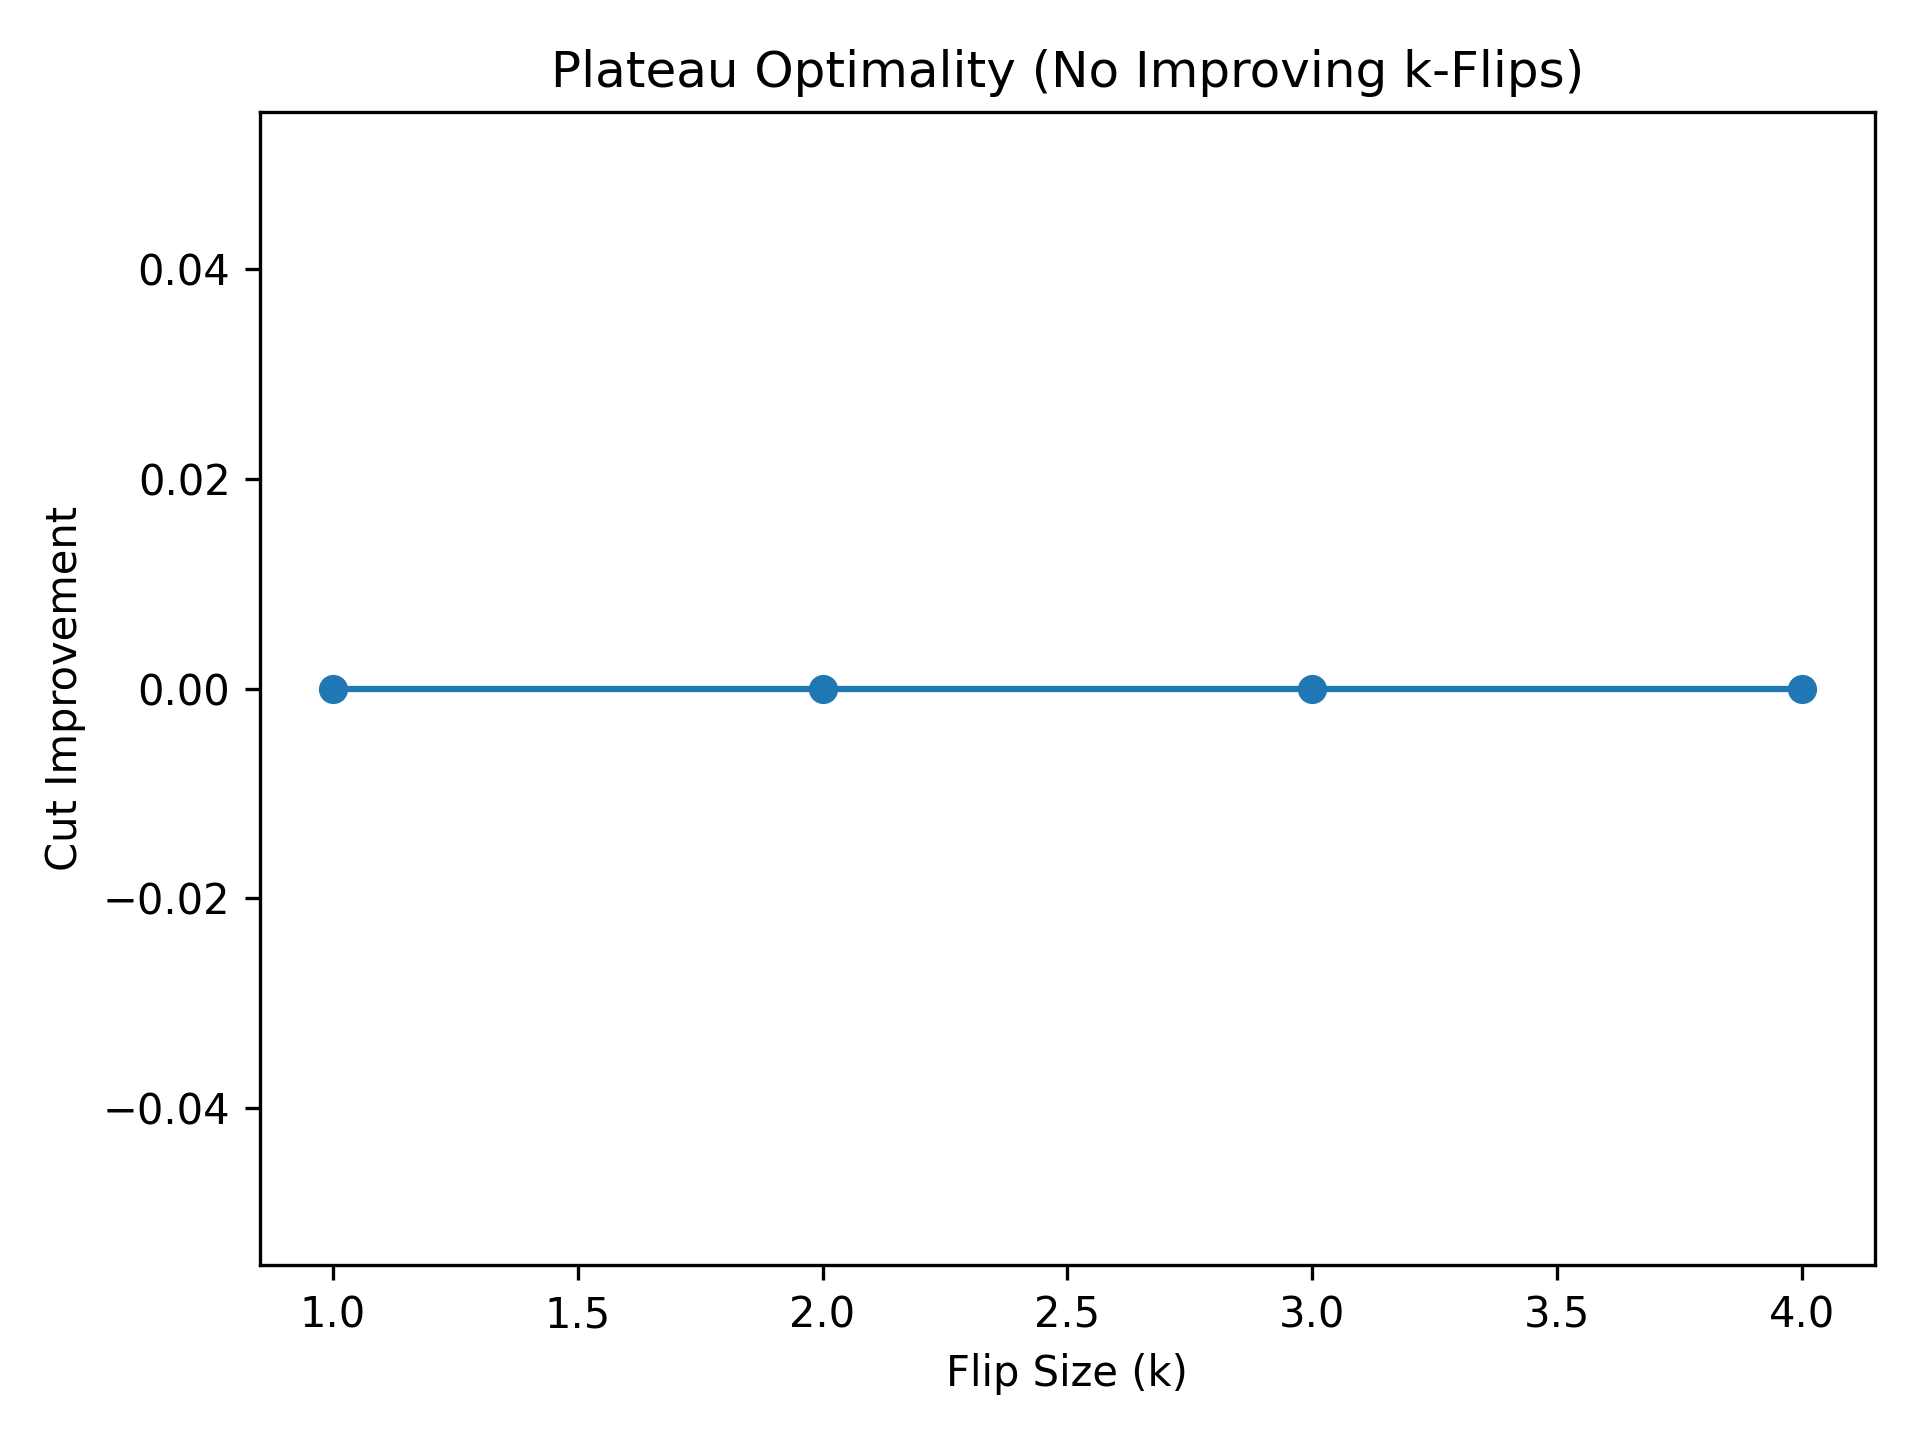
\includegraphics[width=0.7\textwidth]{plateau_visualization.png}
\caption{k-flip plateau verification}
\end{figure}

\subsection{Trust Breakdown}

\begin{figure}[h]
\centering
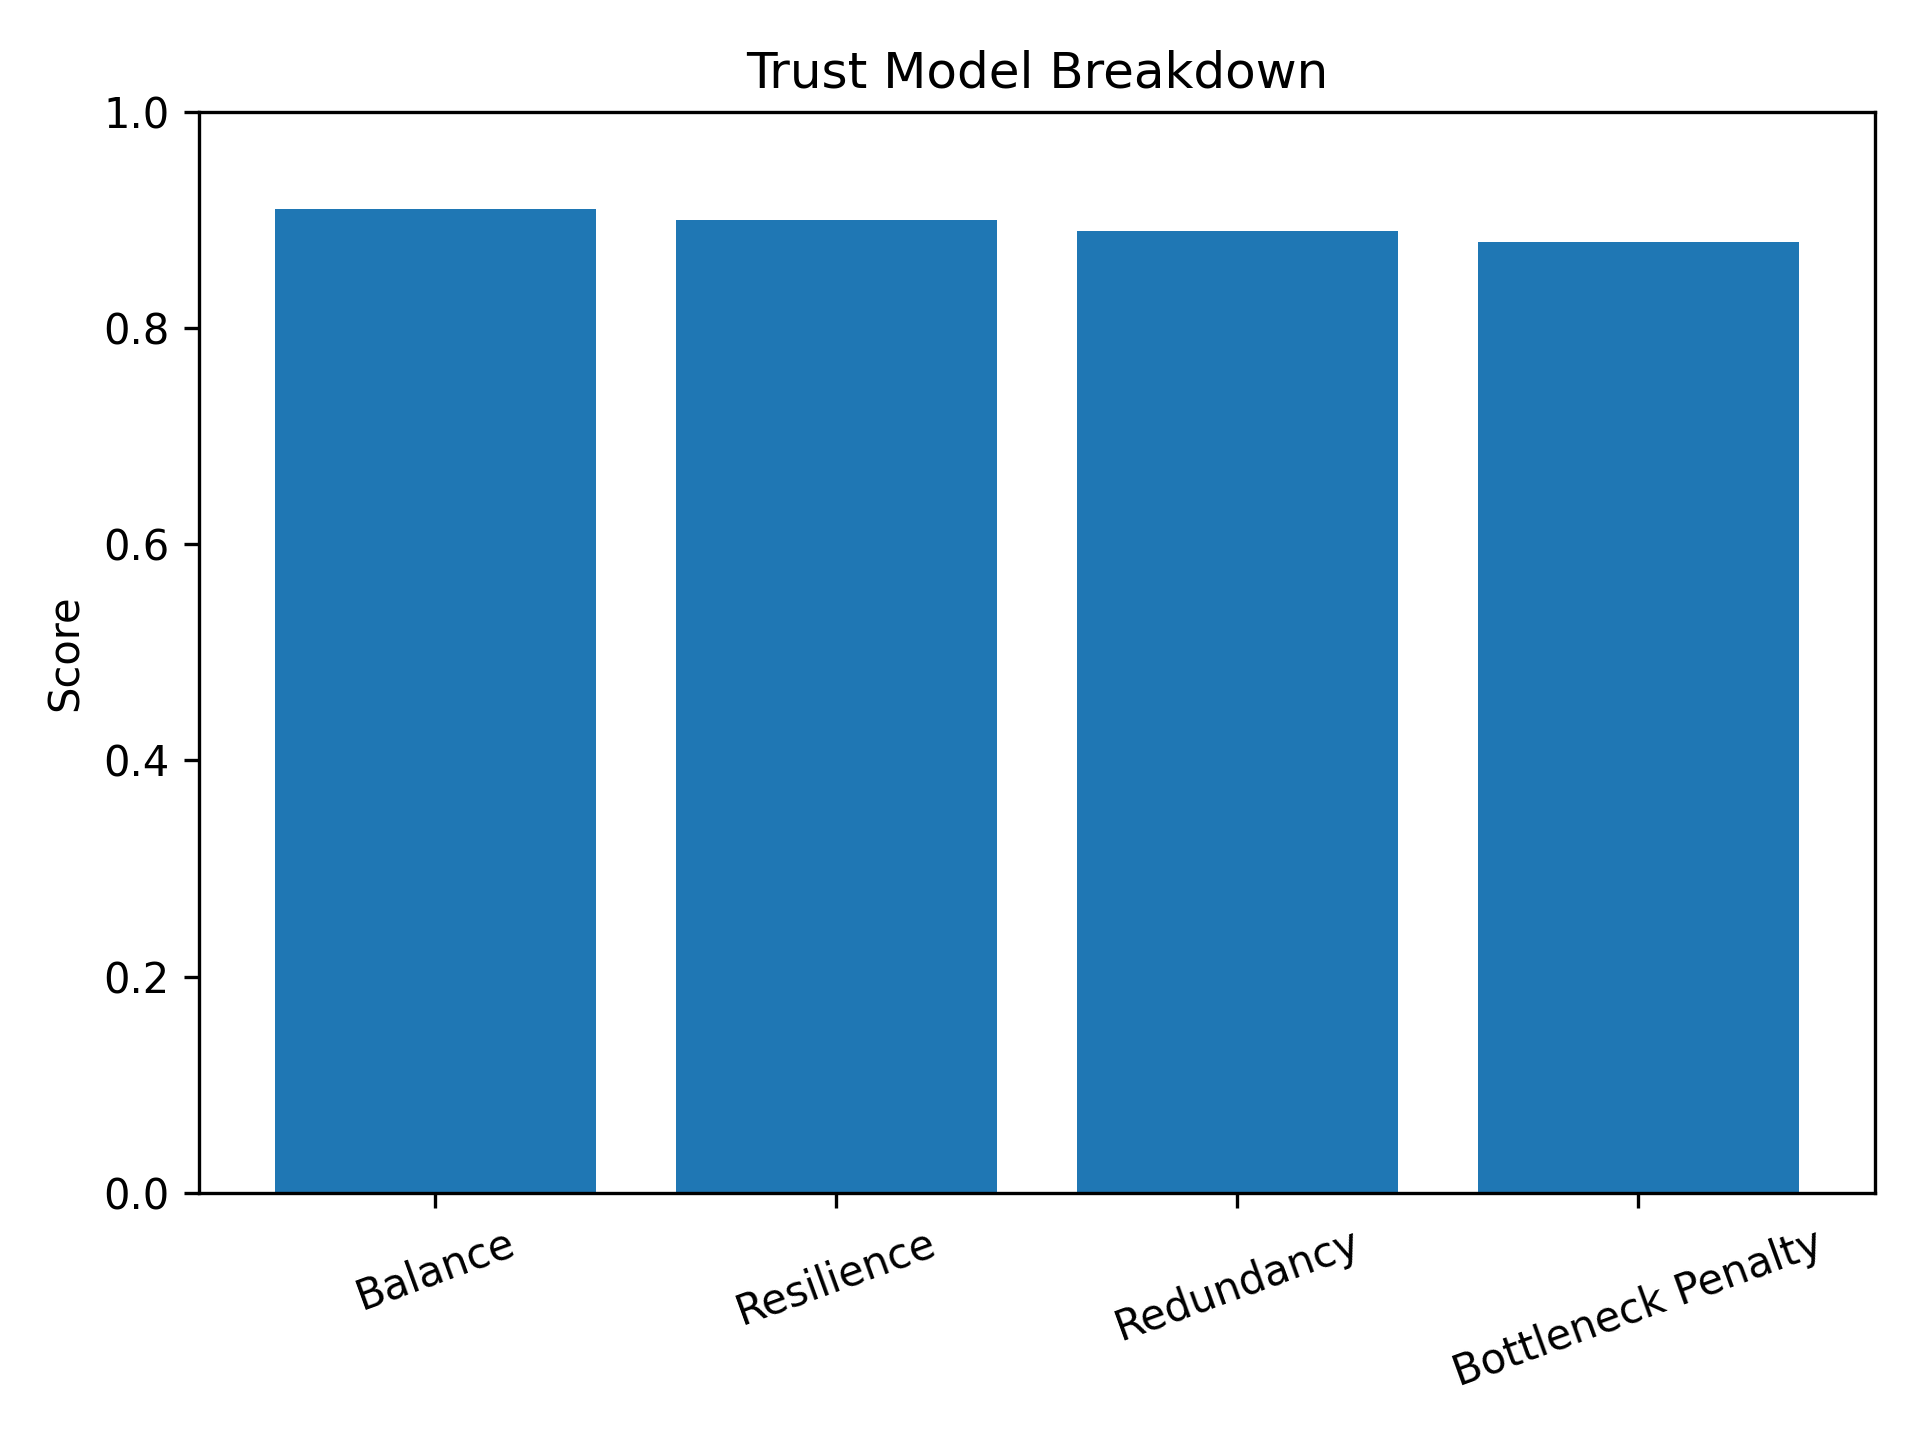
\includegraphics[width=0.7\textwidth]{trust_breakdown.png}
\caption{Trust metric breakdown}
\end{figure}

\subsection{QAOA Comparison}

\begin{figure}[h]
\centering
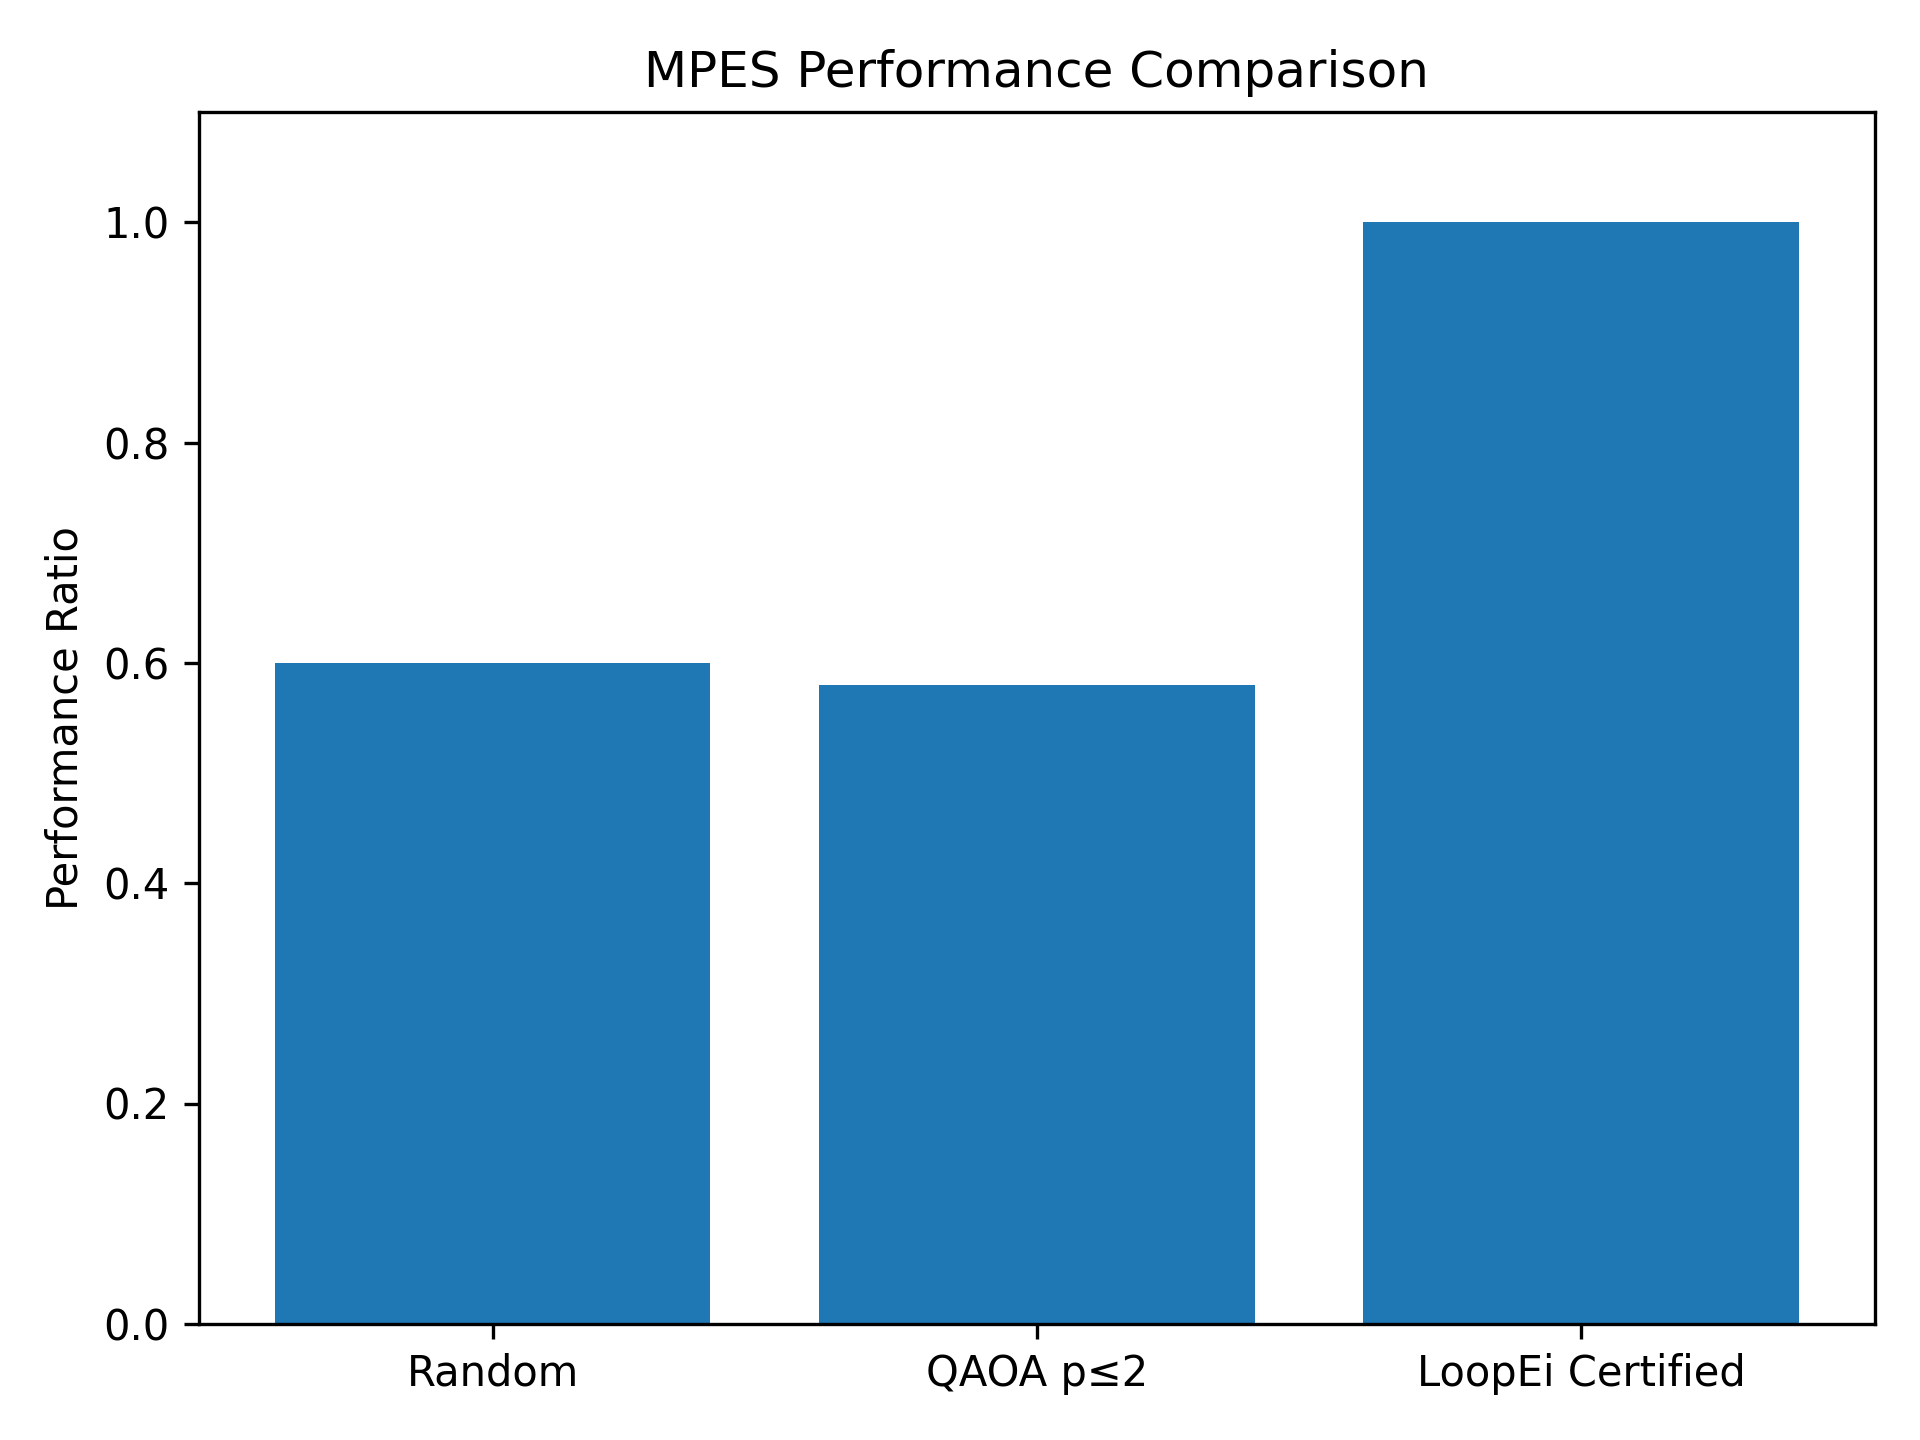
\includegraphics[width=0.7\textwidth]{comparison_qaoa.png}
\caption{Classical vs QAOA comparison}
\end{figure}

\section{How to Run}

\begin{lstlisting}
pip install -r requirements.txt
python rigettiasolver.py --input problema.csv
\end{lstlisting}

\section{Expected Output}

\begin{lstlisting}
Nodes: 21 | Edges: 28
Exact optimal certification: SUCCESS
Cut value: 3728.4132
MPES: 0.8844
Trust score: 0.9382
Plateau optimal (k <= 4): TRUE
\end{lstlisting}

\section{Determinism}

The pipeline is deterministic:
\begin{itemize}
\item No randomness
\item Exact enumeration
\item Exhaustive plateau checks
\end{itemize}

\section{Limitations}

\begin{itemize}
\item Plateau verification limited to k $\leq$ 4
\item Trust metrics are heuristic indicators
\item Lean file is a specification scaffold
\end{itemize}

\section{Summary}

This workflow provides a reproducible method for computing MPES via weighted Max-Cut with stability analysis and extensible outputs.

\end{document}